\documentclass[12pt]{article}

% look up all the included packages online
%--------------------------------------------------%
\usepackage{graphicx}		% include figures
\usepackage{subcaption} 	% for subfigure captions
\usepackage{float}			% [H] float command
\usepackage{sidecap}		% make sidecaptions with SCfigure
\usepackage[space]{grffile}	% allow spaces in paths
\usepackage{wrapfig}		% wrap figures with wrapfigure
%--------------------------------------------------%

% ignore this, for demo purposes only
\usepackage[english]{babel}
\usepackage{blindtext}

% useful packages for tables, especially if you 
% are doing sequences
\usepackage{booktabs}
\usepackage{multirow}
\usepackage{seqsplit}
\usepackage{array}
\usepackage{longtable}
\usepackage{tabularx}
\usepackage{tabu} 

% specify where your images are located
% you can have multiple locations to look up
% separate different paths by a comma (,) with NO
% space
%-----------------------------------------------%
\graphicspath{{./},{./images/},{./other_images/}}
%-----------------------------------------------%

\begin{document}

% just like table of contents, you can have a 
% table of contents for figures and tables
%-------------%
\listoffigures
\listoftables
%-------------%

\section{Figures}

% basic code to place a figure
% change the dimension of the figure
% also use the sidecap package to make the caption
% on the side versus just to top or bottom
%-------------------------------------------%
\begin{figure}[H]

\includegraphics[width=\linewidth]{img1.jpg}
\caption{Your first figure placement}
\end{figure}
%-------------------------------------------%

% play around with wrapfigure to incorporate
% text and figure placement
%-------------------------------------------%
\blindtext % <- ignore this, random text
\begin{wrapfigure}{r}{0.5\textwidth}
	\begin{center}
		
\includegraphics[width=0.48\textwidth]{img2.jpg}
	\end{center}
	\caption{Wrapped around}
\end{wrapfigure}
\blindtext % <- ignore this, random text
%-------------------------------------------%

% assemble a big figure with subfigures
%-------------------------------------------%
\begin{figure}[H]
    \centering
    \begin{subfigure}[b]{0.3\textwidth}
        
\includegraphics[width=\textwidth]{img1.jpg}
        \caption{caption 1}
    \end{subfigure}
	% space
    \begin{subfigure}[b]{0.3\textwidth}
        
\includegraphics[width=\textwidth]{img2.jpg}
        \caption{caption 2}
    \end{subfigure}
    % space
    \begin{subfigure}[b]{0.3\textwidth}
        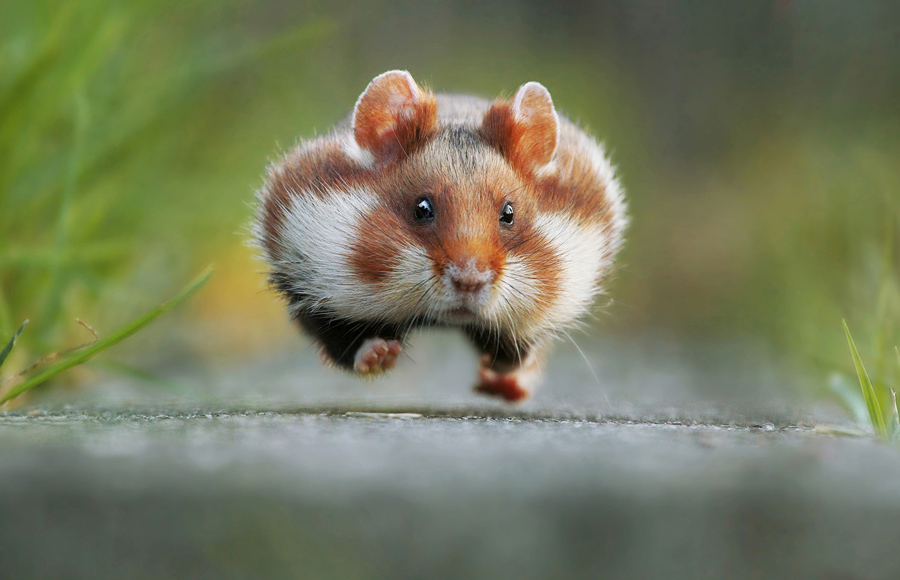
\includegraphics[width=\textwidth]{img3.jpg}
        \caption{caption 3}
    \end{subfigure}
    \caption{Pictures of cute things}
\end{figure}
%-------------------------------------------%

\section{Tables}
%--------------------------------------------------%
% use this website to convert excel to latex tables
% https://www.tablesgenerator.com/
%--------------------------------------------------%
% table 1 without borders and all centered
\begin{table}[H]
	\begin{center}
		\begin{tabular}{ c c c }
		cell1 & cell2 & cell3 \\ 
		cell4 & cell5 & cell6 \\  
		cell7 & cell8 & cell9    
		\end{tabular}
	\end{center}	
	\caption{table (naked)}
\end{table}

% table 2 with border
\begin{table}[H]
	\begin{center}
		\begin{tabular}{| c | c | c |}
			\hline
			cell1 & cell2 & cell3 \\
			\hline 
			cell4 & cell5 & cell6 \\  
			\hline
			cell7 & cell8 & cell9 \\
			\hline    
		\end{tabular}
	\end{center}
	\caption{table (bordered)}	
\end{table}

% personal opinion: make it pretty
\begin{table}[H]
	\begin{center}
		\begin{tabular}{ c c c }
		\toprule
		heading1 & heading2 & heading 3 \\
		\midrule		
		cell1 & cell2 & cell3 \\ 
		cell4 & cell5 & cell6 \\  
		cell7 & cell8 & cell9 \\
		\bottomrule   
		\end{tabular}
	\end{center}
	\caption{table (booktabbed)}	
\end{table}

\end{document}